\documentclass[12pt,a4paper]{article} %,fleqn
\usepackage{Diplo}
\usepackage[utf8]{inputenc} 
\usepackage[russian]{babel}

\usepackage[left=3cm,right=1.5cm,
top=2cm,bottom=2cm]{geometry}

\usepackage{comment}
\usepackage{hyperref}
\usepackage[square, comma, sort&compress, numbers]{natbib}
\newtheorem{definition}{Определение}
\newtheorem{theorem}{Теорема}
\newtheorem{utv}{Утверждение}

\graphicspath{{../pics/}}

\begin{document}
	
\vskip 3mm

\setcounter{page}{1}
%%%%%%%% Титульный лист %%%%%%%%%%%%%%%%%%%%%%%%%%%%%%%%%
\begin{center}
	\thispagestyle{empty}
	
	{ Министерство науки и высшего образования Российской Федерации\\}

	
	
	{ Московский Физико-технический институт \\}
	
	{ (Государственный Университет) \\}
	
	{ Факультет управления и прикладной математики  \\}
	
	{ Кафедра Интеллектуальных систем\\}
	
	{при Вычислительном Центре им. А.А.Дородницына РАН\\ [4cm]}
	
	{ \bf \Large Выпускная квалификационная работа\\}
	
	{ \bf \Large{"Разработка метода выделения века как параметрической кривой на изображении глаза"\\[1cm]} }
	
	{\bf {Студента 4-го курса Ефремова Сергея Владимировича}\\[3cm]}
	
\end{center}

\begin{flushright}
	\bf{Научный руководитель}\\
	\bf{д-р техн. наук Матвеев И. А.}\\[4cm]
\end{flushright}


\begin{center}
	Москва, 2020
\end{center}
%%%%%%%%%%%%%%%%%%%%%%%%%%%%%%%%%%%%%%%%%%%%%%%%%%%%%%%%%%%%%%%%

\newpage
\begin{abstract}

Рассматривается задача выделения века как параметрической кривой на изображении глаза. Исследованы предложенные ранее схемы решения этой проблемы, на основе изученных материалов разработан подход по его выделению как параболы с помощью поиска максимума на множестве проекций. Предложен, реализован и протестирован алгоритм, основанный на параболическом преобразовании и преобразовании Радона.	

\end{abstract}

\newpage
\tableofcontents
 


\newpage
\section{Введение}

На сегодняшний день можно с уверенностью говорить о том, что биометрические технологии идентификации вошли в нашу жизнь и используются во всех сферах человеческой деятельности, в том числе и в системах контроля. Существует целый ряд биометрических модальностей, позволяющих идентифицировать человека: рисунок папиллярных линий пальца, радужка глаза, походка, голос, почерк. Такое разнообразие методов объясняется тем, что при богатстве потенциальных сценариев использования биометрических модальностей, каждая из них может быть использована по-разному. Применение биометрических технологий уже активно осуществляется при проведении платежных операций в банковской сфере, особо нуждающейся в защите данных. Здесь они заменяют уже ставшие традиционными методы идентификации пользователей: ПИН-коды, пароли и т.д. Биометрические технологии имеют широкую перспективу использования, так как обладают целым рядом неоспоримых преимуществ, cреди которых можно выделить неотчуждаемость. Например, пароль может быть передан или украден третим лицом, и система все равно идентифицирует его как исходного пользователя, тогда как биометрическими модальностями труднее воспользоваться другому человеку или украсть без ведома обладателя. 

Использование биометрических систем настолько повсеместно, что обыватель даже не замечает, как часто и повсеместно ими пользуется. Так, для разблокировки мобильных устройств, применяется отпечаток пальца, снимок лица или радужки. Еще одним преимуществом биометрических систем считается удобство взаимодействия с ними пользователя. Их эффективность работы основывается на способности обработки поступающих данных с учетом изменчивости состояния и условий окружающей среды. То есть, даже в случае значительных искажений параметров входных данных, в связи с изменчивостью состояний (например, ухудшение условий освещенности, затемнение ресницами, отвод взгляда), системы биометрической идентификации, использующие изображения глаза, должны выдавать корректный результат и аутентифицировать пользователя адекватно. Также неоспоримо важным фактором для эффективности систем такого рода, является необходимость работы в условиях ограниченности не только вычислительных ресурсов, но и времени, требующегося на распознавание. 

Благодаря стремительному развитию технологий, с каждым днём все больше расширяется сфера практического применения технических средств цифровой обработки изображений. Одним из направлений стало распознавание человека на основе изображения глаза~(рис.~\ref{fig:glaz}). Эта идея не нова, ещё в 1936 году офтальмологи \cite{Medic} предложили использовать радужную оболочку глаза для распознавания. Далее исследователями всего мира разрабатывались различные методы распознавания человека по его радужной оболочке, но по-настоящему сильный рост интереса произошел только в начале XXI века. Это объясняется качественными изменения условий жизни общества: эволюция средств регистрирования и обработки изображений, необходимость распознавания личности в связи с террористической угрозой~\cite{Conf3, Terr, Tech}. Наряду с идентификацией обработка изображения радужки применяется в медицинских целях, где также важно выделение области интереса. 

\begin{figure}[h]
	
	\centering
	
	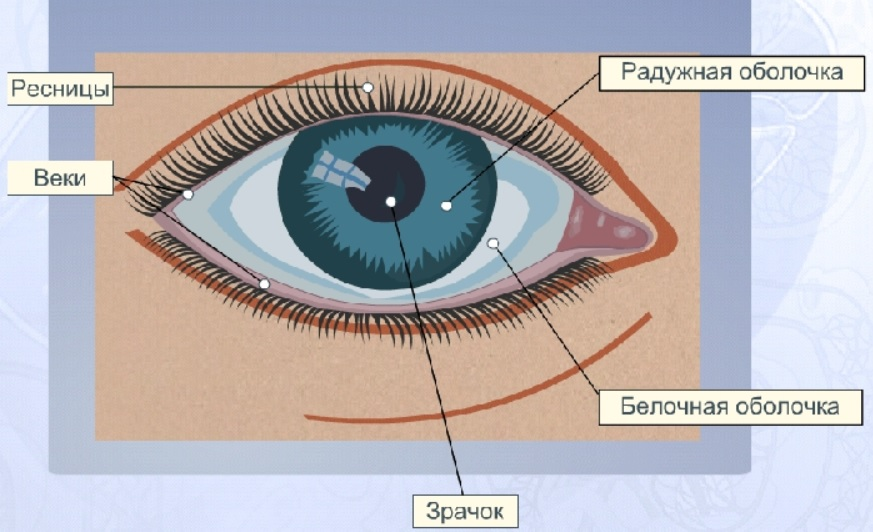
\includegraphics[width=0.6\linewidth]{glaz.jpg}
	
	\caption{Внешнее строение глаза.}
	
	\label{fig:glaz}
	
\end{figure}

Однако получить качественное и обособленное изображение радужки на практике не так просто, и важной задачей оказывается необходимость корректно определять границы глаза, задаваемые веками. Исследования в этом направлении породили различные модели, которые также используют в биометрических системах распознавания, поскольку уточнение границ и исключение нерелевантных областей оказывает значительное влияние на точность результата.

В ходе данного исследования разработан метод выделения века как параметрической кривой на изображении глаза. Он состоит в определении параметров кривой максимизацией суммы вертикального градиента яркости, рассматриваемого в окрестности века.
 

\newpage
\subsection{Цели и задачи работы}

\textbf{Цель и задачи исследования.} Целью исследования является построение модели, позволяющей определять коэффициенты параболы, задающей положение верхнего века и улучшить качество выделения по сравнению с существующими моделями. Для реализации этой цели были поставлены следующие задачи:
\begin{itemize}
	\item изучить существующие подходы к решению задачи выделения века на изображении глаза;
	\item изучить существующие алгоритмы решения этой задачи;
	\item создать метод предобработки данных;
	\item реализовать алгоритмическую часть модели, построенной на идее оптимизации и градиентного анализа;
	\item сравнить полученные результаты с результатами существующих алгоритмов.
\end{itemize}

\bigskip

\textbf{Научная новизна.} Используется новый подход к определению коэффициентов параболы, с помощью поиска максимума на множестве проекций.

\bigskip

\textbf{Методы исследования.} Алгоритмы реализованы на языке программирования C++ с использованием библиотеки OpenCV~3.4.

\bigskip

\textbf{Практическая ценность.} Полученная модель может быть использована в качестве встраиваемого модуля. Например, с её помощью можно:
\begin{itemize}
	\item определять границы зрачка глаза для повышения точности идентификации по радужке;
	\item дополнять существующие биометрические системы с помощью признаков не только радужки, но и линии века, получая более высокое качество распознавания.
\end{itemize}
%%%%%%%%%%%%%%%%%%%%%%%%%%%%%%%%%%%%%%%%%%%%%%%%%%%%%


\newpage
\section{Постановка задачи}


\subsection{Задача выделения века}\label{task}
В алгоритмах идентификации, использующих радужку, чаще всего начинают с определения границы радужка-склера \cite{Adam_1, Daugman, Matv} или нормализуют радужку (рис.~\ref{fig:glaz3}) \cite{Min}, а лишь только потом определяют границу века. Это приводит к необходимости выполнять большое количество дополнительных вычислений. Рассмотрим только те методы, в которых для детектирования века необходимо заранее определить не более чем положение зрачка или радужки.

\begin{figure}[h]
	
	\centering
	
	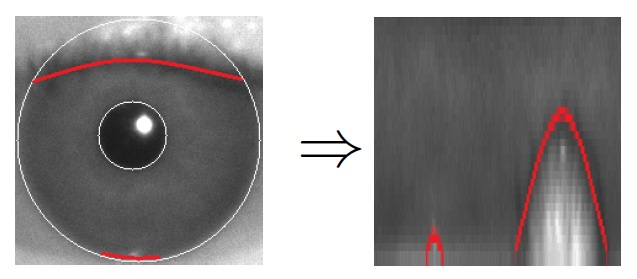
\includegraphics[width=0.8\linewidth]{glaz3.jpg}
	
	\caption{Определение положения века.}
	
	\label{fig:glaz3}
	
\end{figure}

Можно определить два ключевых этапа в произвольном алгоритме детектирования века на изображении глаза, один из которых ~--- предобработка изображения, а второй~--- локализация века. Как правило, исследователи работают только над одним из этапов, в то время как второй заимствуют из уже ранее написанных работ, предлагая новые комбинации предобработка/локализация, которые ранее не были описаны в научной литературе. Предложенный метод сравнивается с наиболее успешными комбинациями, показывающими наиболее точный результат при тестировании.

Для нахождения границы века в~\cite{Wildes} предложено использовать в качестве первого шага выделение границ на изображении, а затем для локализации века~--- преобразование~Хафа. 

В \cite{Daugman} используется сглаживание изображения с применением фильтра Гаусса и интегродифференциальный оператор
(IDO) для того, чтобы найти контуры на изображении, в том числе нижнее и верхнее веко.

Ещё один метод выделения века предложен в \cite{KKX}, для предообработки используется одномерный фильтр пиковой формы, хорошо удаляющий шум от ресниц, а для локализации IDO.

Интуитивно понятный метод изложен в \cite{Masek}. Его идея заключается в разделении области радужки и века горизонтальными прямыми, их положение вдоль вертикальной оси определялось значением максимального отклика после осуществления свёртки изображения с использованием фильтра Собела. Эта же свёртка применяется в \cite{KP} в сочетании с IDO. 

В исследованиях \cite{Adam_2, Adam_1} используется анизотропная диффузия для погашения шумов при предобработке, фильтр Собела для веделения границ и преобразование Хафа для параболических кривых. 

Для выделения границ в \cite{Yang} предложен асимметричный оператор Кэнни и для локилизации~--- аппроксимация параболической кривой с помощью метода наименьших квадратов. 

В качестве одного из методов определения границ века также можно выделить метод адаптивных контуров, предложенный в \cite{Smirn}. Его основная идея~--- задать модель контура последовательностью точек и оптимизировать функционал на этом контуре, таким образом добиваясь его эволюции.

Почти все изложенные выше методы базируются на необходимости наличия дополнительных внешних условий или требований к качеству изображения, поэтому не всегда отличаются устойчивостью в условиях постоянно изменяющегося окружения. 

\subsection{Формальная постановка задачи}

Пусть $f(x, y)$~--- множество точек, задающих линию века на изображении глаза и
\newline $y=a(x-x_0)^2 + y_0$~--- уравнение аппроксимирующей параболы. Также пусть площадь круга радужки со зрачком~--- $S$.
Обозначим площадь области в круге радужки, в которой парабола выше линиии века как $E_2$, и площадь области, в которой выше веко~--- $E_1$~(рис.~\ref{fig:glaz8}). Тогда суть задачи~--- найти такие коэффициенты $(a,x_0,y_0)$:
\begin{gather}\label{minimax}
	(a,x_0, y_0)=\argmin_{(a,x_0,y_0)}\left<\max{\Bigl\{\frac{E_1}{S}, \frac{E_2}{S}\Bigr\}}\right>.
\end{gather}

\begin{figure}[h]
	
	\centering
	
	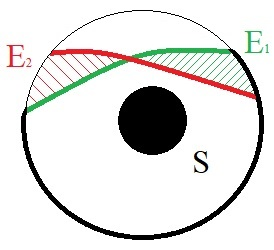
\includegraphics[width=0.28\linewidth]{glaz8.jpg}
	
	\caption{Веко~--- зеленая линия и аппроксимирующая парабола~--- красная.}
	
	\label{fig:glaz8}
	
\end{figure}
\newpage
\subsection{Оценка качества}

В качестве еще одного метода оценки полученного результата предлагается рассмотреть отклонение вершины параболы от эталона. Ожидается, что это будет самая высокая точка кривой века (рис.~\ref{fig:glaz2}).

\begin{figure}[h]
	
	\centering
	
	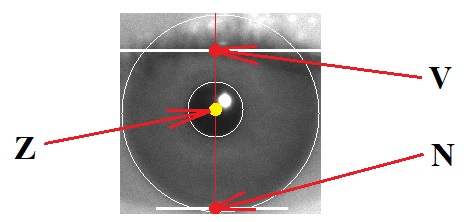
\includegraphics[width=0.6\linewidth]{glaz2.jpg}
	
	\caption{Определение положения века: $V$ и $N$~--- точки, соответствующие положениям верхнего и нижнего век; $Z$~--- центр зрачка.}
	
	\label{fig:glaz2}
	
\end{figure}

Тогда анализируемая метрика примет вид:
\begin{gather}\label{dist}
dist = \sqrt{\frac{(y-y_0)^2}{y_0^2}+\frac{(x-x_0)^2}{x_0^2}},
\end{gather}
где $(x_0, y_0)$~--- экспертная разметка вершины, а $(x,y)$~--- экспериментальная.
%%%%%%%%%%%%%%%%%%%%%%%%%%%%%%%%%%%%%%%%%%%%%%%%%%%%%

\newpage
\section{Обзор существующих методов}
\subsection{Модели аппроксимации века}

\subsubsection{Эллиптический контур века}

Один из возможных способов приблизить линию века~--- описать её с помощью эллиптической кривой. Эта модель основана на предположении, что глазное яблоко имеет сферическую форму:
\begin{gather}\label{sphear}
	x^2+y^2+z^2= R^2.
\end{gather}

Такое предположение приводит к модели, основанной на открытости глаза. Степень открытости~--- угловое положение века относительно центра сферы. Тогда кривую века можно получить как пересечение сферы глазного яблока с плоскостью проходящей через ось $x$ с углом $\varphi$ относительно оси $z$ (рис.~\ref{fig:glaz4}). Уравнение этой плоскости имеет вид:
\begin{gather}\label{el1}
	\tan{\varphi}= \frac{y}{z}.
\end{gather}

А кривая пересечения, моделирующая веко, задается эллиптической кривой:
\begin{gather}\label{el2}
	x^2+\frac{y^2}{\sin{\varphi}^2}=R^2.
\end{gather}

\begin{figure}[h]
	
	\centering
	
	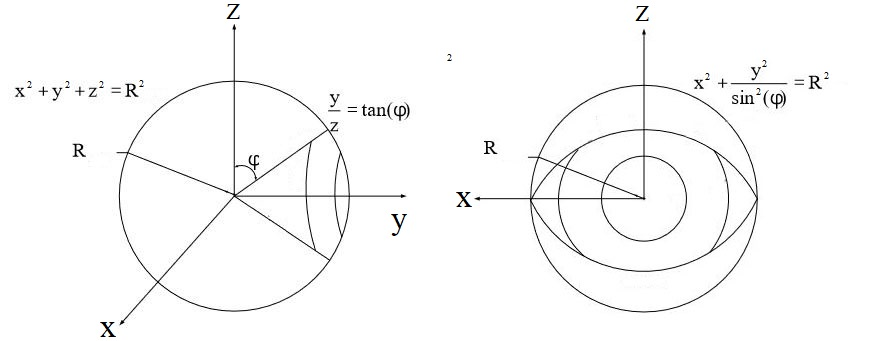
\includegraphics[width=0.8\linewidth]{glaz4.jpg}
	
	\caption{Вид сбоку и спереди эллиптического контура века.}
	
	\label{fig:glaz4}
	
\end{figure}


\subsubsection{Параболический контур века}

На практике оказывается, что определять кривую века как пересечение плоскости и сферы довольно грубо. Эмпирическим путем было установлено, что форма века глаза человека гораздо лучше аппроксимируется квадратичной параболой~(рис.~\ref{fig:glaz5}). Тогда уравнение параметрической кривой, задающее контур века принимает вид:
\begin{gather}\label{par1}
	y = a(x-x_0)^2 + y_0.
\end{gather}

\begin{figure}[h]
	
	\centering
	
	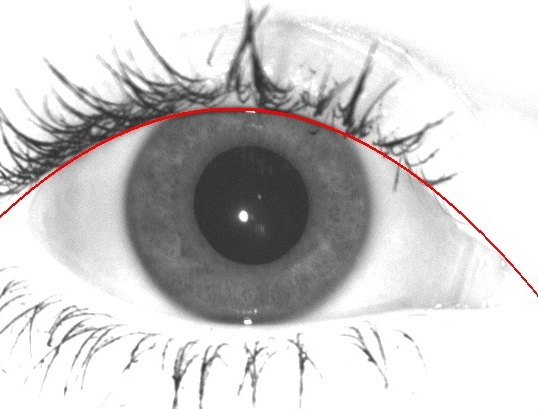
\includegraphics[width=0.5\linewidth]{glaz5.jpg}
	
	\caption{Пример параболического контура века на изображении глаза.}
	
	\label{fig:glaz5}
	
\end{figure}

\newpage
\subsection{Методы выделения контуров}

Практически все методы выделения контуров основываются на перепадах сигнала яркости. Наиболее общим способом их поиска является обработка изображения методом скользящего окна, называемого в разной литературе также маской, фильтром, ядром или шаблоном. Оно представляет из себя некую прямоугольную матрицу, накладываемую на группу пикселей исходного изображения. Элементы такой матрицы называют коэффициентами, а разного рода преобразования над ней~--- фильтрацией или пространственной фильтрацией(рис.~\ref{fig:prost_filt}).

\begin{figure}[h]
	
	\centering
	
	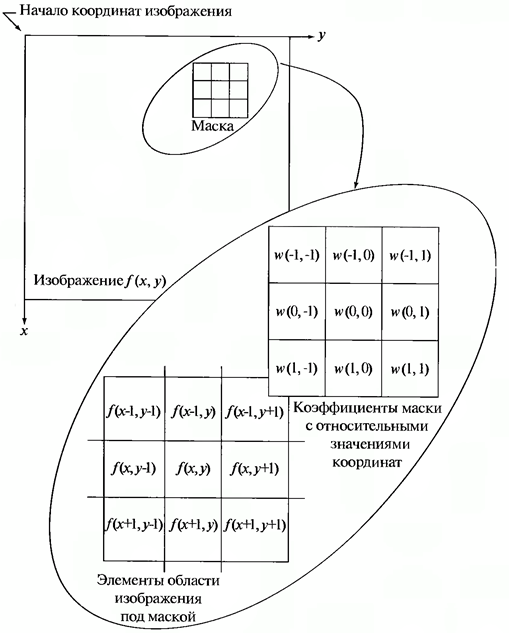
\includegraphics[width=0.5\linewidth]{prost_filt.jpg}
	
	\caption{Схема пространственной фильтрации.}
	
	\label{fig:prost_filt}
	
\end{figure}

\newpage

 Метод основан на перемещении фильтра от точки к точке, вычисляется отклик для каждой из них. Для случая линейной пространственной фильтрации значение задается суммой произведения коэффициентов маски на соответствующие значения яркостей в точках, покрытых маской. Так, для квадратной маски размерности $3\times3$ отклик $R$ линейной фильтрации в точке $(x, y)$ изображения на рис.~\ref{fig:prost_filt} определится как сумма произведений значений маски на значнения пикселей под маской:
\begin{gather}\label{3.1}
R = \sum\limits_{s=-1}^{1}
{\sum\limits_{t=-1}^{1}{w(s,t)f(x+s, y+t)}}.
\end{gather}

\subsubsection{Производные 1-го и 2-го порядков}

Для определения направления и величины перепада яркости чаще всего применяют градиент изображения $\boldsymbol{\nabla}f$, определяемый в точке $(x,y)$ как вектор:
\begin{gather}\label{grad}
	\boldsymbol{\nabla}{f} \equiv \text{grad}(f)\equiv
	\begin{bmatrix} g_x \\ g_y \end{bmatrix}=
	\begin{bmatrix} \frac{\partial f}{\partial x} \\ \frac{\partial f}{\partial y}
	\end{bmatrix}.
\end{gather}

Важным геометрическим свойством градиента является тот факт, что его направление совпадает с направлением максимальной скорости изменения функции f в точке $(x, y)$. Направление вектора градиента задаётся углом между направлением вектора $\bigtriangledown \mathbf{f}$ и осью~$x$:
\begin{gather}\label{grad_alpha}
	\alpha(x, y) = \text{arctg}\left(\frac{g_y}{g_x}\right).
\end{gather}

Направление контура в произвольной точке $(x,y)$ таким образом получается перпендекулярно направлению $\alpha(x,y)$ вектора градиента в этой точке(рис.~\ref{fig:grad}).


\begin{figure}[h]
	
	\centering
	
	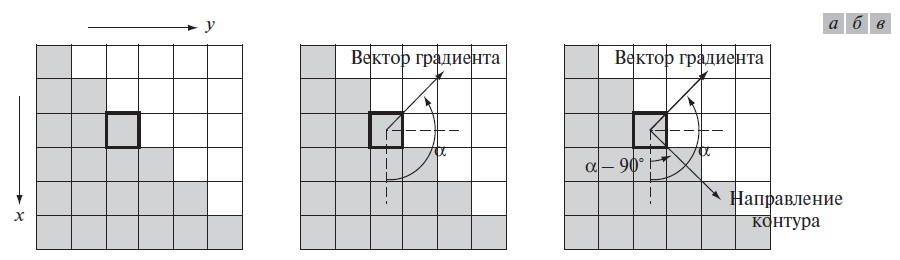
\includegraphics[width=0.7\linewidth]{grad.jpg}
	
	\caption{Применение градиента для нахождения границ контуров на изображении.}
	
	\label{fig:grad}
	
\end{figure}

При работе с изображениями функция яркости имеет дискретную природу, поэтому вместо производных первого и второго порядка используются их дискретные аналоги.

Первая производная одномерной функции может быть задана как разность значений соседних элементов:
\begin{gather}\label{first}
	\frac{\partial f}{\partial x}=
	f(x+1) - f(x).
\end{gather}

Аналогично вторая производная определяется как разность соседних значений первой производной:
\begin{gather}\label{second}
	\frac{\partial^2 f}{\partial^2 x}=
	f(x+1) + f(x-1) -2f(x).
\end{gather}

Нетрудно заметить, что по факту эти преобразования задают маски фильтрации для первой и второй производной вдоль вертикальной координатной оси~(рис.~\ref{fig:grad_mask}).
\begin{figure}[h]
	
	\centering
	
	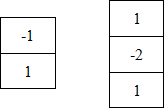
\includegraphics[width=0.2\linewidth]{grad_mask.jpg}
	
	\caption{Маски фильтрации для первой и второй производной вдоль вертикальной координатной оси.}
	
	\label{fig:grad_mask}
	
\end{figure}

Однако способ дискретно приблизить производную, описанный выше, не единственный. Можно, например, использовать маски размером $3\times3$. Далее описаны другие вариации градиентных операторов.

\subsubsection{Оператор Робертса}

Обозначим область изображения размером $3\times 3$ и значения яркостей каждой из ее точек в соответствии с рис.~\ref{fig:grad_mask_3}.

\begin{figure}[h]
	
	\centering
	
	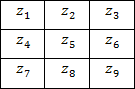
\includegraphics[width=0.2\linewidth]{grad_mask_3.jpg}
	
	\caption{Яркости в области $3\times3$ на изображении.}
	
	\label{fig:grad_mask_3}
	
\end{figure}

Один из возможных способов нахождения первых частных производных в точке~$z_5$ состоит в применении перекрестного оператора Робертса:
\begin{gather}\label{grad_mask_3}
	g_x = \frac{\partial f}{\partial x} = (z_9-z_5),\\
	g_y = \frac{\partial f}{\partial y} = (z_8-z_6).
\end{gather}

Такое преобразование задает маски фильтрации на рис.~\ref{fig:grad_mask_rob} соответственно.

\begin{figure}[h]
	
	\centering
	
	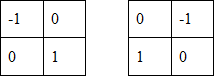
\includegraphics[width=0.25\linewidth]{grad_mask_rob.jpg}
	
	\caption{Маски оператора Робертса.}
	
	\label{fig:grad_mask_rob}
	
\end{figure}

Основным преимуществом данного градиентного оператора является высокая скорость обработки изображения, но зачастую устойчивость оставляет желать лучшего. 

\subsubsection{Оператор Превитта}

Используем обозначения рис.~\ref{fig:grad_mask_3}. Тогда оператор Превитта может быть задан выражениями:
\begin{gather}\label{grad_mask_prev}
	g_x = \frac{\partial f}{\partial x} = (z_7+z_8+z_9)-(z_1+z_2+z_3),\\
	g_y = \frac{\partial f}{\partial y} = (z_3+z_6+z_9)-(z_1+z_4+z_7).
\end{gather}

Маска этого градиентного оператора имеет вид, изображённый на рис.~\ref{fig:grad_mask_prev}.

\begin{figure}[h]
	
	\centering
	
	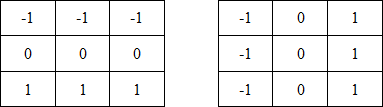
\includegraphics[width=0.4\linewidth]{grad_mask_prev.jpg}
	
	\caption{Маски оператора Превитта.}
	
	\label{fig:grad_mask_prev}
	
\end{figure}

\subsubsection{Оператор Собеля}

Небольшое изменение формул ~(\ref{grad_mask_prev}) в виде использования весового коэффициента~$2$ для средних элементов, позволяет уменьшить эффект сглаживания для функции градиента:
\begin{gather}\label{grad_mask_sob}
	g_x = \frac{\partial f}{\partial x} = (z_7+2z_8+z_9)-(z_1+2z_2+z_3),\\
	g_y = \frac{\partial f}{\partial y} = (z_3+2z_6+z_9)-(z_1+2z_4+z_7).
\end{gather}

Маски, используемые оператором Собеля, отображены на рис.~\ref{fig:grad_mask_sob}.

\begin{figure}[h]
	
	\centering
	
	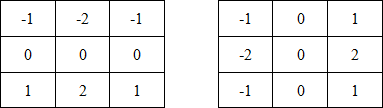
\includegraphics[width=0.4\linewidth]{grad_mask_sob.jpg}
	
	\caption{Маски оператора Собеля.}
	
	\label{fig:grad_mask_sob}
	
\end{figure}

Стоит отметить, что у каждой из градиентных масок, описанных выше, сумма весовых коэффициентов равна нулю, то есть эти операторы будут давать нулевой отклик на областях постоянной яркости, как и следовало ожидать от дифференциального оператора.

\subsubsection{Преобразование Хафа}

Рассмотренные выше методы применимы, когда имеется дополнительная информация о положении исследуемых объектов на изображении. Зачастую таких данных нет и приходится исходить из заранее заданных глобальных свойств. Ниже изложен метод, основанный на выяснении того, лежат ли множества пикселей на кривой заранее заданной формы.
Рассмотрим случай, когда искомая фигура изначально имеет форму прямой, и воспользуемся преобразованием Хафа для её поиска.
Рассмотрим точку~$(x_i, y_i)$ исходного изображения и общее уравнение прямой на плоскости:~$y = ax+b$. Через точку~$(x_i, y_i)$ проходит бесконечное множество прямых, удовлетворяющих уравнению: $y_i = ax_i+b$. Перепишем это уравнение в виде:~$b = x_i a - y_i$ и перейдём систему координат $Oab$, называемую пространством параметров. Очевидно, что в нём для заданной пары~$(x_i, y_i)$ существует уравнение единственной прямой. Более того для каждой пары $(x_i, y_i)$,$(x_j, y_j)$ точек в исходном пространстве, в пространстве параметров существует единственная точка $(a', b')$, находящаяся на пересечении соотвествующих для точек прямых пространства параметров и задающая прямую, на которой лежат эти точки в исходном пространстве(рис.~\ref{fig:param_haf}).

\begin{figure}[h]
	
	\centering
	
	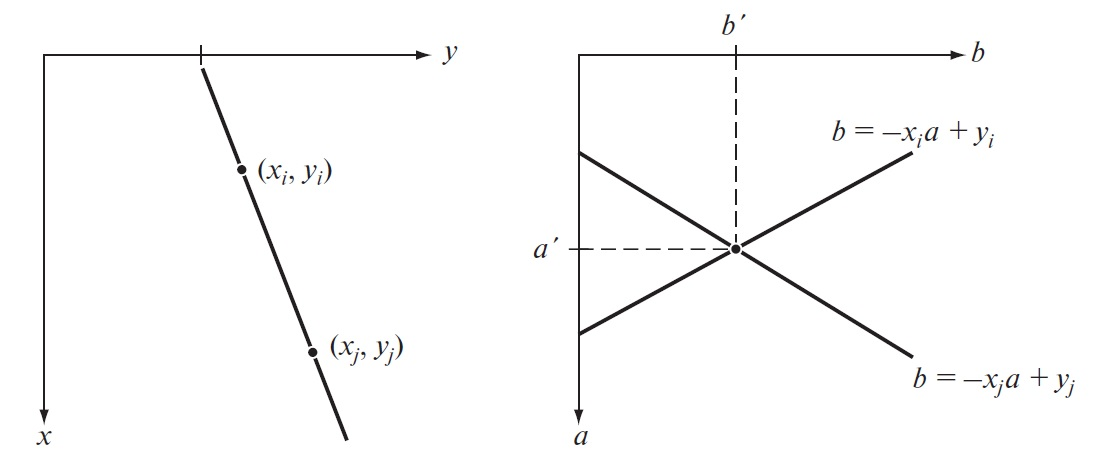
\includegraphics[width=0.6\linewidth]{param_haf.jpg}
	
	\caption{Исходная плоскость~($xy$), пространство параметров~($ab$).}
	
	\label{fig:param_haf}
	
\end{figure}

Проблема использования такого перехода проявляется при попытке отобразить прямую близкую к вертикальной, так как ее угловой коэффициент $a$ стремится к бесконечности. Чтобы обойти данную трудность прямую представляют с помощью нормали:
\begin{gather}\label{norm1}
	x\cos{\Theta} + y\sin{\Theta} = \rho.
\end{gather}

Геометрическую интерпретацию параметров~$\rho$~и~$\Theta$ можно увидеть на рис.~\ref{fig:norm}-а. Каждая синусоида на рис.~\ref{fig:norm}-б представляет семейство прямых, проходящих через конкретную точку $(x_k, y_k)$ на исходной плоскости $xy$. Точка перечения $(\rho'\Theta')$ на этом рисунке соответствует прямой, проходящей через точки $(x_i, y_i)$ и $x_j, y_j$ на рис.~\ref{fig:norm}-а.

\begin{figure}[h]
	
	\centering
	
	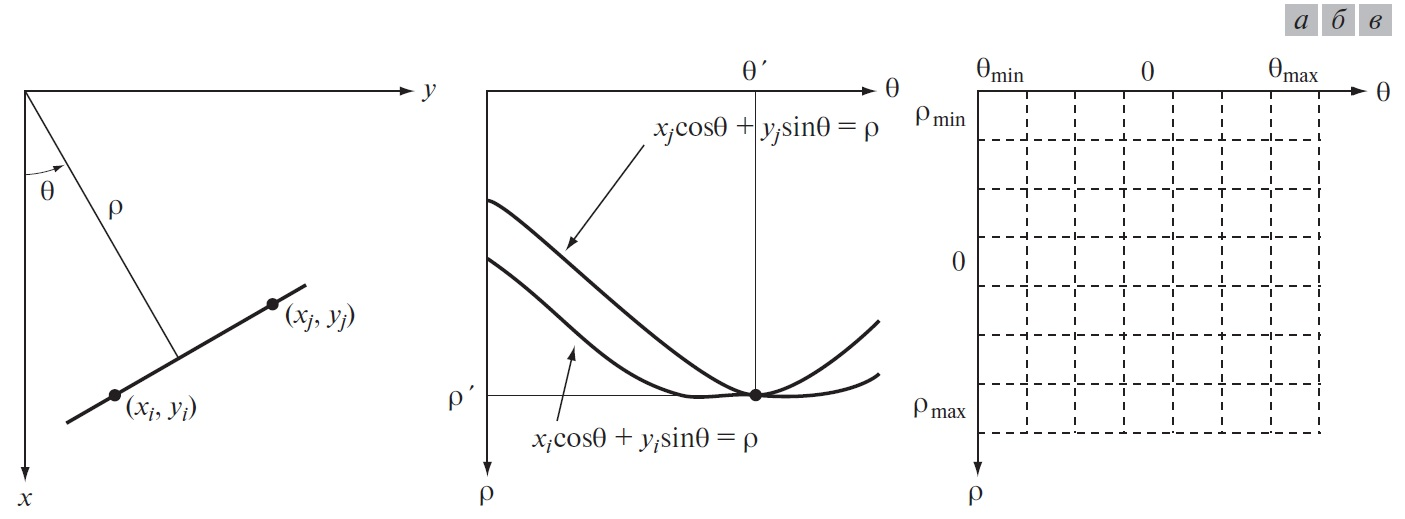
\includegraphics[width=0.8\linewidth]{norm.jpg}
	
	\caption{(а)~Представление прямой на исходной плоскости с помощью параметров нормали $(\rho, \Theta)$. 
	(б)~Синусоиды на плоскости $\rho \Theta$.
	(в)~Разбиение плоскости $\rho \Theta$ на ячейки накопления.}
	
	\label{fig:norm}
	
\end{figure}

Осуществив преобразование Хафа, далее предлагается разбить пространство параметров $\rho \Theta$ на так называемые ячейки накопления, как показано на рис.~\ref{fig:norm}-в. Затем для каждой точки $(x_k, y_k)$ исходной плоскости перебираем возможные значения для параметра $\Theta$ и находим соотвествующее ему значение $\rho = x_k\cos{\Theta}+y_k\sin{\Theta}$. Если выбор значения $\Theta_p$ приводит к решению $\rho_q$, то увеличиваем значение ячейки $A(p,q)$ на~1. После выполнения этого алгоритма значение $A(p,q)=Q$ означает, что на исходной плоскости находится $Q$ точек лежащих на прямой $\rho_p = x_k\cos{\Theta_q}+y_k\sin{\Theta_q}$.
Отсюда и находят прямые контуры поиском локальных максимумов. 

Аналогичным образом можно применять преобразование Хафа к любой функции вида $g(v,c) = 0$, где $v$~--- вектор координат, а $c$~--- вектор коэффициентов.
Так, любое коническое сечение, в частности парабола, может быть задано уравнением в полярных координатах:

\begin{gather}\label{conic}
	\rho = \frac{de}{1\pm e\cos{\Theta}}
\end{gather}

или
\begin{gather}\label{conic2}
	\rho = \frac{de}{1\pm e\sin{\Theta}},
\end{gather}
где $e$~--- эксцентриситет и $d$~--- кратчайшее расстояние между фокусом и директрисой. Для конических сечений эксцентриситет имеет разные значения в зависимости от формы кривой. Для эллипса он лежит в диапазоне: $0<e<1$, для гиперболы~--- $e>1$, а для параболы~--- $e = 1$, её далее и рассмотрим.

Парабола может быть определена как геометрическое множество точек, равноудалённых от неподвижной точки, называемой фокусом, и прямой, называемой директрисой~(рис.~\ref{fig:hough_parab}). Эта парабола описывается уравнением:
\begin{gather}\label{parab_equ}
	(y-y_0)^2 = 4a(x-x_0)
\end{gather}
 или
 \begin{gather}\label{parab_equ_2}
 	Ay^2+By+C=x
 \end{gather}
\begin{figure}[h]
	
	\centering
	
	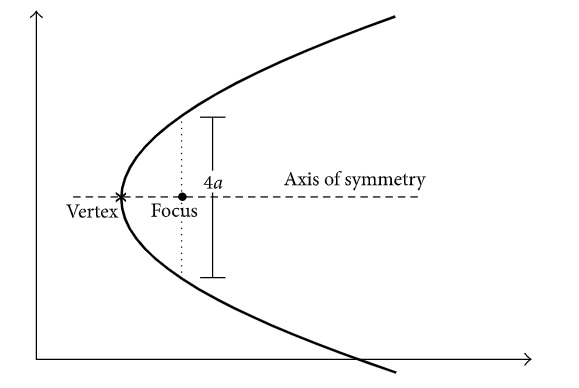
\includegraphics[width=0.6\linewidth]{hough_parab.jpg}
	
	\caption{Парабола.}
	
	\label{fig:hough_parab}
	
\end{figure}

Коэффициенты можно вычислить по формулам~\cite{Hough_Parab}: 
 \begin{gather}\label{parab_equ_3}
	A=\frac{y_k(x_j-x_i)+y_j(x_i-x_k)+y_i(x_k-x_j)}{(y_i-y_j)(y_i-y_k)(y_j-y_k)},\\
	B=\frac{y_k^2(x_j-x_i)+y_j^2(x_i-x_k)+y_i^2(x_k-x_j)}{(y_i-y_j)(y_i-y_k)(y_j-y_k)},\\
	C= \frac{y_jy_k(y_j-y_k)x_i+y_ky_i(y_k-y_i)x_j+y_iy_j(y_i-y_j)x_k}{(y_i-y_j)(y_i-y_k)(y_j-y_k)}.
\end{gather}

Таким образом, перебрав все тройки точек, переходим в пространство коэффициентов, в котором, аналогично пространству для прямых, считаем значения в ячейках накопления, но уже в трехмерных.

Наконец, можно получить значения координат вершины и апертуры параболы:
\begin{gather}\label{parab_equ_4}
	x_0 = -\frac{B}{2A},\\
	y_0 = C-\frac{B^2}{4A},\\
	4a=\frac{1}{A}.
\end{gather}


\subsubsection{Преобразование Радона}

Рассмотрим простейший случай преобразования Радона, а именно случай двух переменных. Исходим из предположения, что $f(x,y)$ определена на всей плоскости и достаточно быстро убывает на бесконечности. Последнее условие необходимо для сходимости несобственных интегралов. Тогда преобразованием Радона $f(x,y)$ называется функция~\cite{Radon}:
\begin{gather}\label{radon}
	Rf(s, \alpha) = \int_{-\infty}^{\infty}{f(x(z),y(z))} = \int_{-\infty}^{\infty}{f(s\cos{\alpha}+z\sin{\alpha}, s\sin{\alpha}-z\cos{\alpha})dz}
\end{gather}

Геометрический смысл этого преобразования~--- это интеграл от функции вдоль прямой, перпендикулярной вектору $\vec{n}=(\cos{\alpha}, \sin{\alpha})$ и проходящей на расстоянии $s$ от начала координат вдоль этого вектора (рис.~\ref{fig:Radon_transform}).
\begin{figure}[h]
	
	\centering
	
	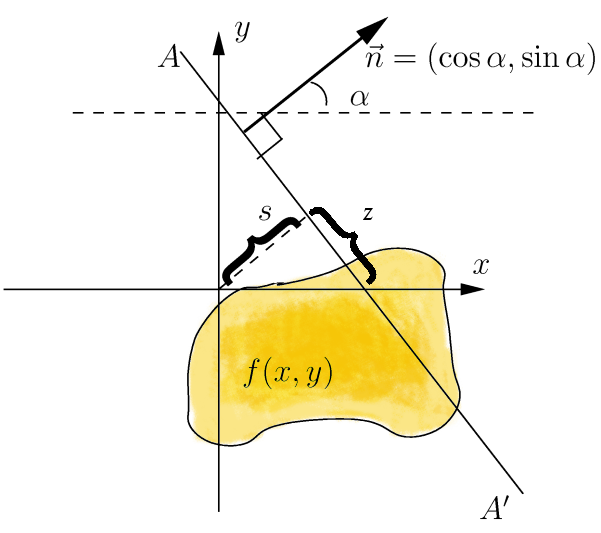
\includegraphics[width=0.5\linewidth]{Radon_transform.jpg}
	
	\caption{Преобразование Радона.}
	
	\label{fig:Radon_transform}
	
\end{figure}

\subsubsection{Интегро-дифференциальный оператор (IDO)}

Оператор, предложенный в \cite{Daugman2}, а затем развитый в \cite{Daugman4, Daugman}, используется в первую очередь для детектирования объектов круглой формы: в оригинале зрачка и радужки. Также предложено детектировать верхние и нижние веки путём настройки поиска контура с кругового на дугообразный~\cite{Daugman}.

Интегро-дифференциальный оператор определяется как:
\begin{gather}\label{ido}
	\max_{r, x_0, y_0}{\left| G_\sigma(r)*\left(\frac{\delta}{\delta r}\right)\int_{r, x_0, y_0}{\frac{I(x,y)}{2\pi r}ds}\right|}.
\end{gather}

При непрерывном применении оператора на изображении максимизируется исследуемый функционал по трём параметрам $(x_0, y_0)$~--- координаты центра и радиус $r$. Ожидается, что границы зрачка и радужки будут максимизировать производную интеграла по круговым границам, так как на них значения интерсивности резко меняются. $G_\sigma(r)$~--- сглаживающая функция. Для век алгоритм аналогичный, только форма искомых контуров будет иметь другой вид. Существенная проблема для данного метода~--- излишняя зашумлённость изображения, которая может породить внезапные перепады у интегрируемого функционала.


\subsubsection{Оператор Кэнни}

Детектор контуров, предложенный в \cite{Canny}, является многоступенчатым алгоритмом обнаружения контуров различной формы и природы. Последовательность действий может быть описана таким образом:

\begin{enumerate}
	\item Применить гауссовский фильтр для сглаживания изображения и удаления шума;
	\item Найти градиенты интенсивности изображения;
	\item Подавить немаксимумы для корректного определения границ;
	\item Применить пороговую фильтрацию для определения потенциальных контуров;
	\item Выделение наиболее весомых контуров.
\end{enumerate}

\textbf{Фильтр Гаусса}

Уравнение, задающее ядро Гауссовского фильтра размера $(2k+1)\times (2k+1)$:
\begin{gather}\label{norm}
	H_{ij}=\frac{1}{2\pi \sigma^2}\exp{\left(\ \frac {-(i-(k+1))^2+(j-(k+1))^2}{2\sigma^2}\right)};~~1\leq i, j \leq(2k+1).
\end{gather}

Очевидно, выбор ядра сглаживания влияет на производительность детектора. Чем больше размер фильтра, тем ниже чувствительность к шуму, но тем больше шансы потерять важную информацию.

\newpage



%%%%%%%%%%%%%%%%%%%%%%%%%%%%%%%%%%%%%%%%%%%%%%%%%%%%%%

\newpage
\section{Описание модели}

 Предложенный в данной работе метод определения положения век основан на применении вертикального градиента с последующими параболическим преобразованим и преобразованием Радона(рис.~\ref{fig:map})).

\begin{figure}[h]
	
	\centering
	
	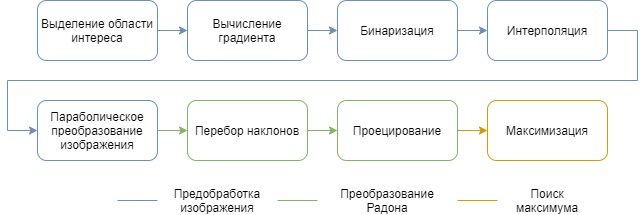
\includegraphics[width=0.8\linewidth]{map.jpg}
	
	\caption{Алгоритм детектирования века на изображении.}
	
	\label{fig:map}
	
\end{figure}

В качестве модели кривой, задающей линию века, выбрана параболическая. Как было описано выше, она позволяет довольно чётко определить границу века и на практике оказывается выигрышной. Таким образом, основной задачей алгоритма становится определить три ключевых параметра: $a, x_0$~и~$y_0$ в~(\ref{parab}), однозначно задающих положение века.
\begin{gather}\label{parab}
	y = a(x-x_0)^2 + y_0.
\end{gather}

\subsection{Этап предобработки изображения}

В качестве входных данных алгоритма, помимо самого изображения глаза, используются координаты центра и радиус зрачка. Нужны эти данные для того, чтобы локализировать веко и ускорить обработку изображения. Высоту рамки области, в которой ищется веко, устанавливаем равной $4 PupR$, где $PupR$~--- радиус зрачка. Область поиска смещаем на $15\%$ от вертикальной координаты центра зрачка. Также оставляем отступ в $5\%$ от горизонтальной координаты центра зрачка слева и справа. Полученный результат локализации изображен на рис.~\ref{fig:glaz6}. Все коэффициенты подобраны опытным путём.

\begin{figure}[h]
	
	\centering
	
	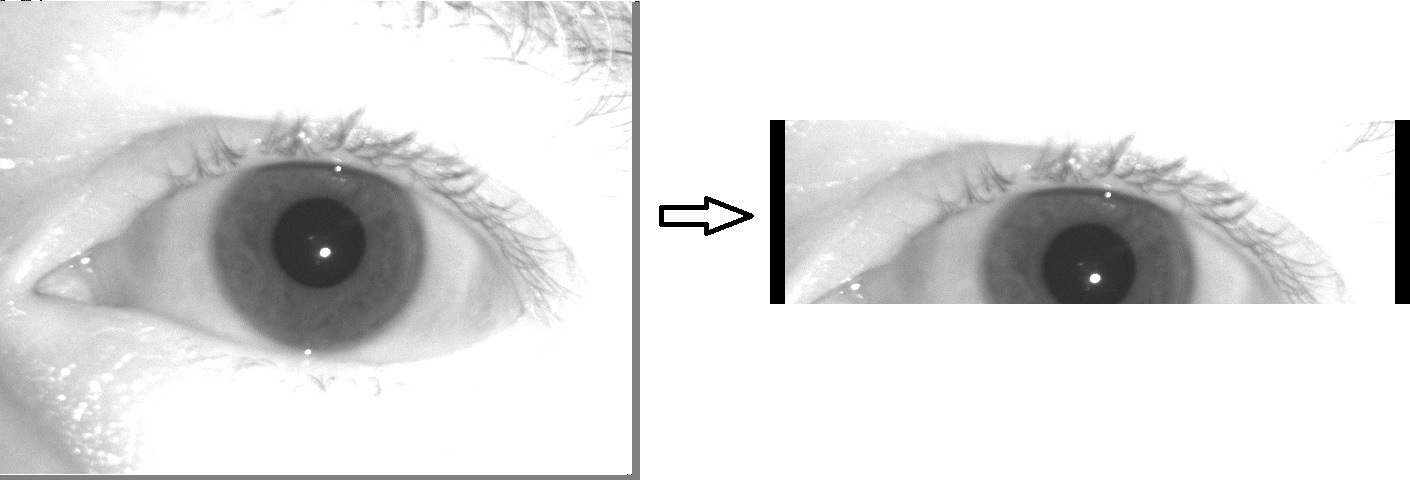
\includegraphics[width=0.8\linewidth]{glaz6.jpg}
	
	\caption{Сужение области поиска.}
	
	\label{fig:glaz6}
	
\end{figure}

Заметим, что линия века на фотографии чаще всего сопровождается резким перепадом яркости по вертикали. Соотвественно легко можно отследить линию века, продифференцировав изображение вдоль вертикальной оси координат (рис.~\ref{fig:glaz7}).

\begin{figure}[h]
	
	\centering
	
	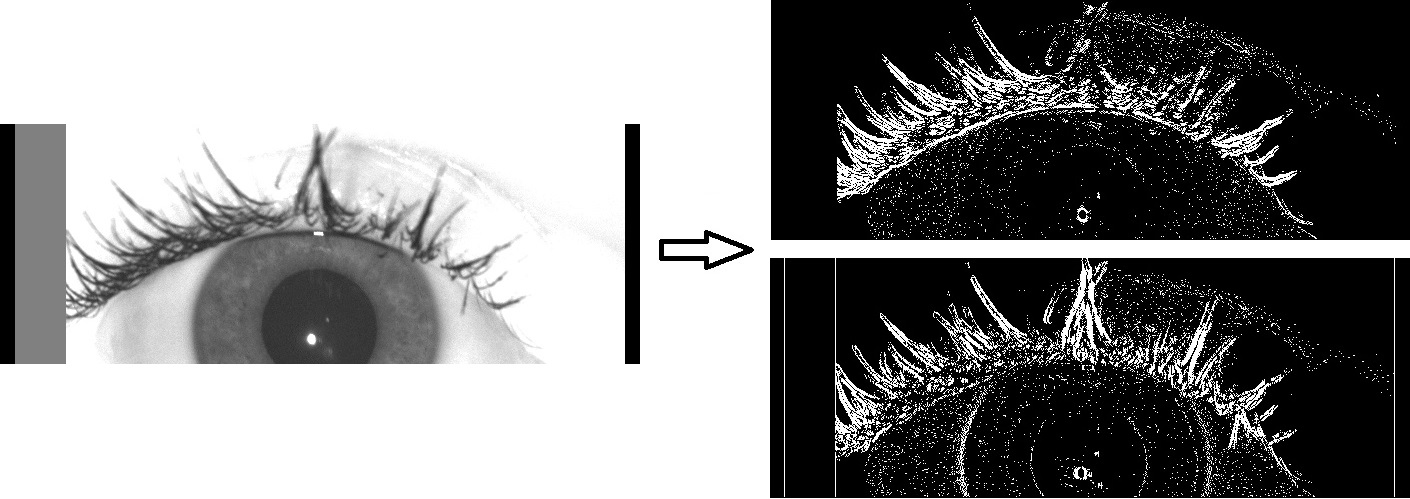
\includegraphics[width=0.8\linewidth]{glaz7.jpg}
	
	\caption{Применение к изображению вертикального и горизонтального градиента с пороговой фильтрацией.}
	
	\label{fig:glaz7}
	
\end{figure}

Помимо непосредственного дифференцирования изображения, также применяем пороговую фильтрацию к модулю разницы значений яркостей в соседних пикселях:
\begin{gather}\label{I_diff}
	 I_d(x,y) = \begin{cases}
	 	255, \text{если}~|I(x,y+1) - I(x,y)|> por,
	 	\\
	 	0, \text{иначе}.
	 \end{cases}
\end{gather}

Величина порогового значения выбрана равной $por=10$ эмпирически.

Заметим, что изображение получилось достаточно зашумлённым. Для того, чтобы это исправить, воспользуемся линейной дискретной интерполяцией. Линейное сглаживание по трём точкам~\cite{Inter}~--- это операция усреднения с помощью интерполяционных многочленов, обеспечивающая возможность получения усредненного значения в точке по заданным соседним. Горизонтальное сглаживание задаётся формулами~\eqref{I_glad}, где $X$~--- число пикселей в строке.
\begin{gather}\label{I_glad}
	I_a(x,y) = \begin{cases}
		\frac{5I(0,y)+2I(1,y)-I(2,y)}{6},~\text{если}~x=0
		\\
		\frac{I(x-1,y)+I(x,y)+I(x+1,y)}{3},~\text{если}~1\leq x\leq X-1
		\\
			\frac{5I(X,y)+2I(X-1,y)-I(X-2,y)}{6},~\text{если}~x=X
	\end{cases}
\end{gather}

Однако, так как мы работаем в бинаризованном пространстве, формула~\eqref{I_glad} приобретает вид:
\begin{gather}\label{I_glad_bin}
	I_{a-bin}(x,y) = \begin{cases}
		I_a, \text{если}~I_a = 255,
		\\
		0, \text{иначе}.
	\end{cases}
\end{gather}

После наложения интерполяционного фильтра изображение приобретает вид рис.~\ref{fig:I_glad}.

\begin{figure}[h]
	
	\centering
	
	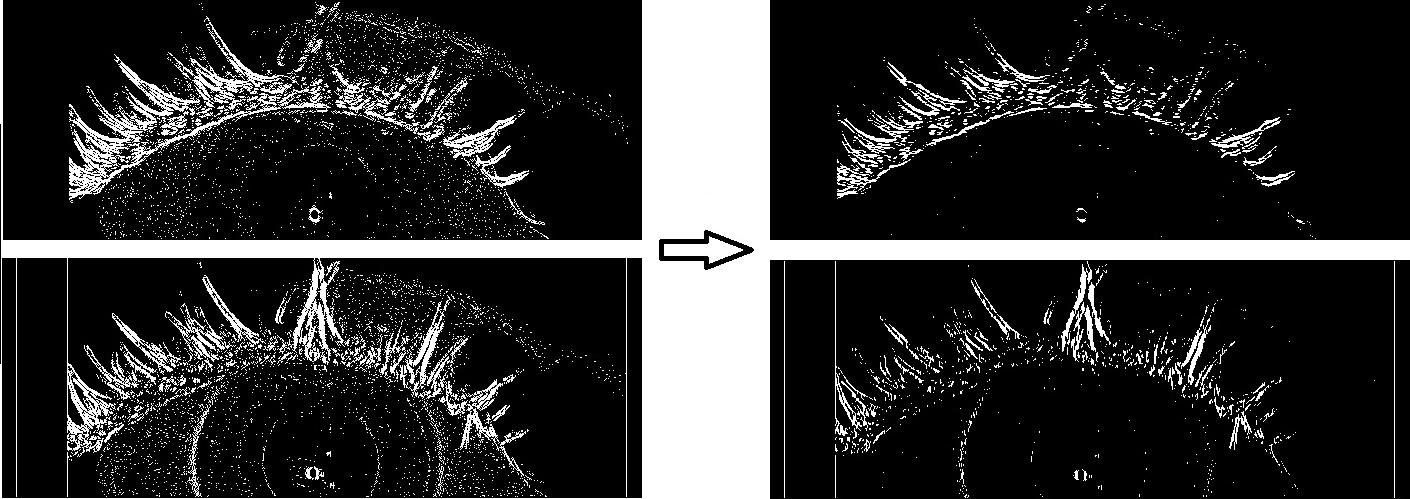
\includegraphics[width=0.8\linewidth]{I_glad.jpg}
	
	\caption{Применение к изображениям вертикального и горизонтального градиента горизонтальной и вертикальной интерполяции соотвественно.}
	
	\label{fig:I_glad}
	
\end{figure}

Заметим, что помимо линии века, очень большой вклад в изображение вертикального градиента всё ещё дают ресницы, однако, на изображении горизонтального градиента веко практически отсутствует, а ресницы всё так же хорошо видны. Воспользуемся этим моментом для уменьшения шума ресниц (рис.~\ref{fig:diff}).
\begin{figure}[h]
	
	\centering
	
	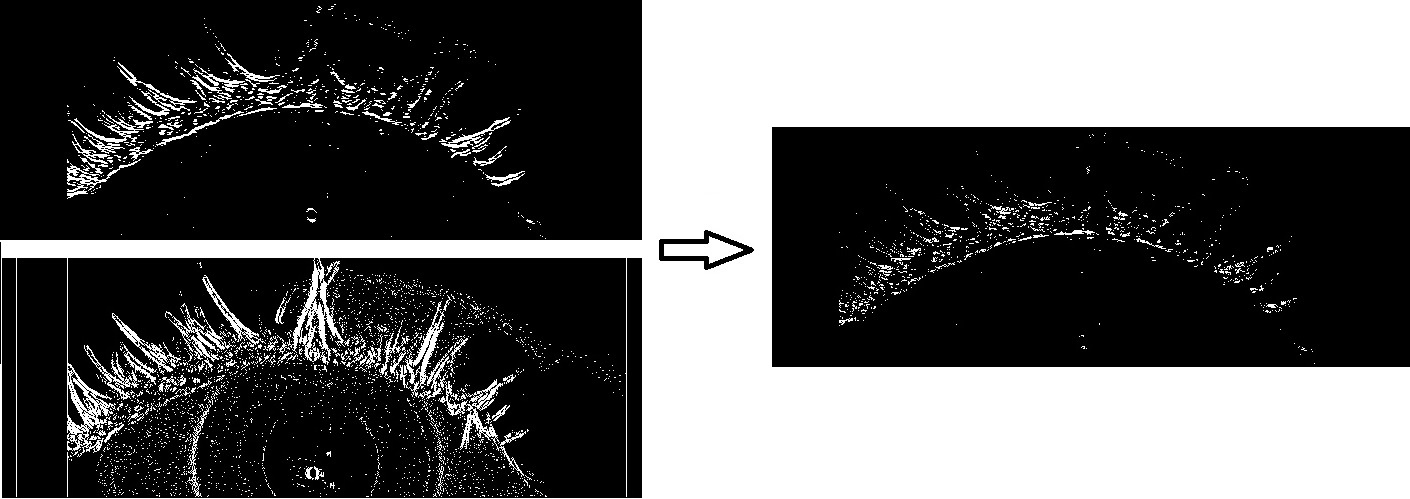
\includegraphics[width=0.8\linewidth]{diff.jpg}
	
	\caption{Уменьшение шума ресниц.}
	
	\label{fig:diff}
	
\end{figure}

Последним этапом предобработки изображения является параболическое преобразование. Его можно представить таким образом:
\begin{gather}\label{parab2}
\begin{cases}
		x' = x,
		\\
		y' = y - ax^2,
	\end{cases}
\end{gather}
где параметр $a$ определяет это преобразование. Заметим, что если в исходном пространстве была задана кривая вида:
\begin{gather}\label{parab3}
 y = a(x-x_0)^2 + y_0,
\end{gather} 
то в пространстве $(y', x')$ она примет вид: 
\begin{gather}\label{parab4}
y = -2ax_0 x + (ax_0^2 + y_0) = bx + c,
\end{gather} 
то есть станет прямой.

Перебирая возможные коэффициенты, мы можем добиться того, чтобы веко приняло форму прямой в конечном пространстве. Пример удачного преобразования на рис.~\ref{fig:parab}.

\begin{figure}[h]
	
	\centering
	
	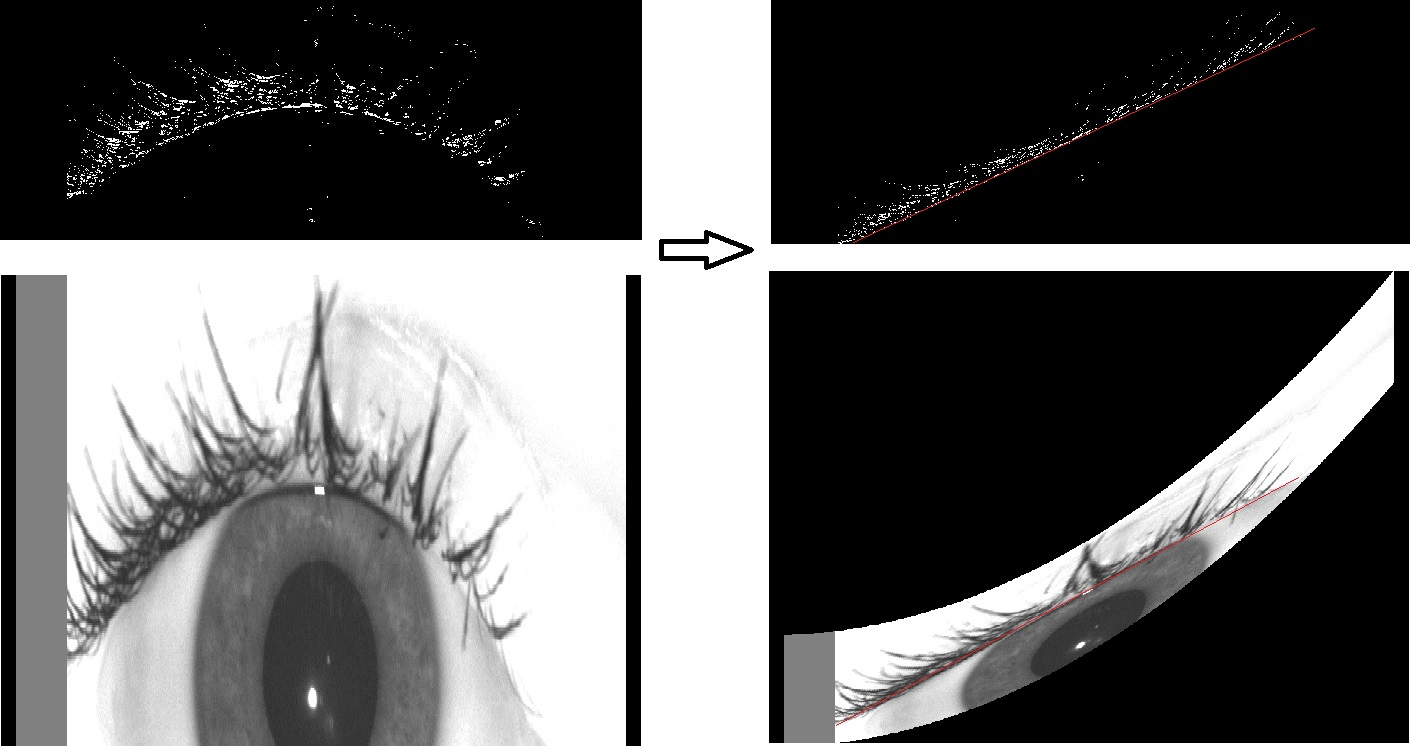
\includegraphics[width=0.8\linewidth]{parab.jpg}
	
	\caption{Параболическое преобразование изображения.}
	
	\label{fig:parab}
	
\end{figure}

Теперь необходимо найти прямую и определить её наклон для корректного определения коэффициентов $x_0$ и $y_0$ для века из уравнения~\eqref{parab3}.
 
\newpage
\subsection{Преобразование Радона}

Перейдём к дискретной интерпретации этого метода. Для того, чтобы применить такое преобразование к изображению, можно разделить его на два этапа: выполнить преобразование поворота и просуммировать построчно значения яркостей. Тогда изменение наклона может быть задано формулой:
\begin{gather}\label{nakl}
	\begin{cases}
		x' = x,
		\\
		y' = y - bx.
	\end{cases}
\end{gather}

Тогда, если прямая изначально имела вид $y=bx+c$, то после преобразования она примет вид $y = c$. Так как шум на изображении всё равно присутствует, далее нужно максимизировать просуммированное значение яркостей вдоль всех строк изображения. Полученный максимум ожидаем в положении последнего искомого коэффициента $c$. Пример преобразования наклона на рис.~\ref{fig:nakl}.

\begin{figure}[h]
	
	\centering
	
	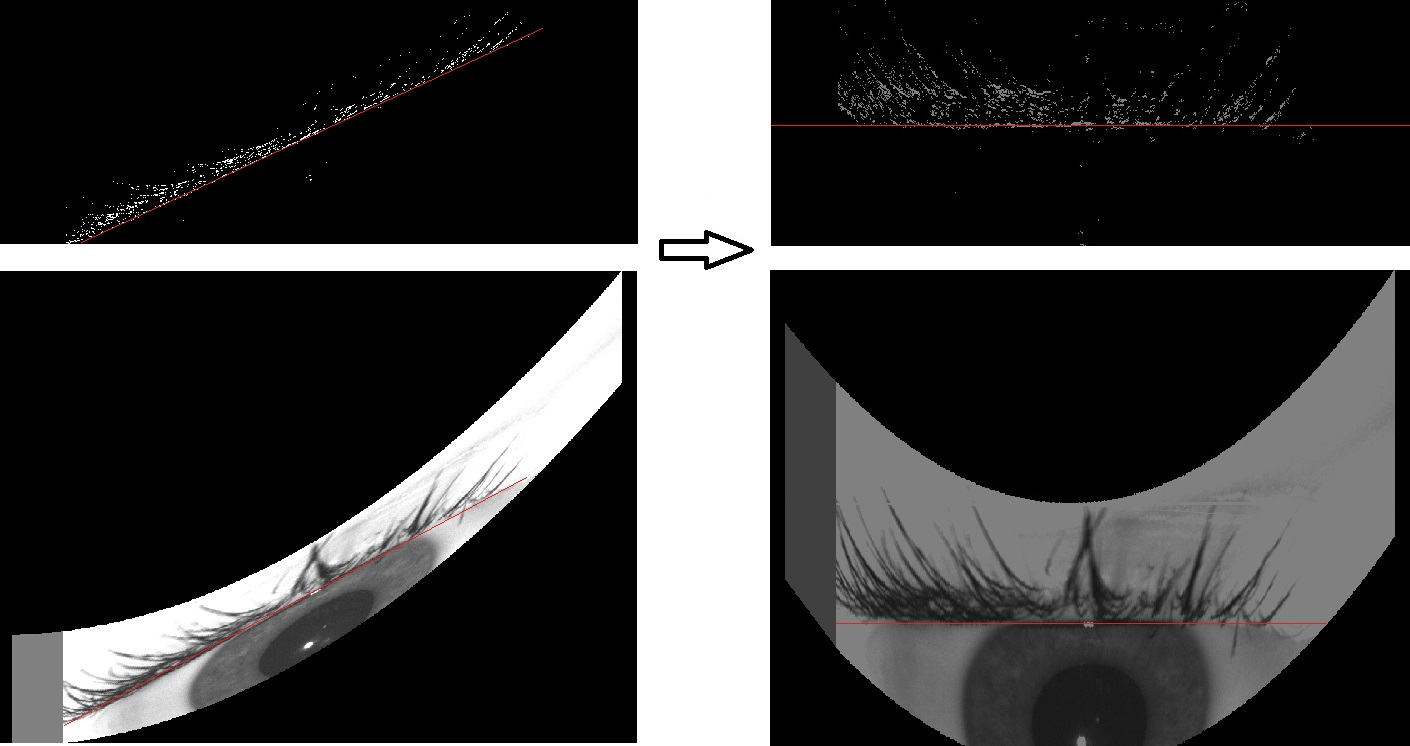
\includegraphics[width=0.8\linewidth]{nakl.jpg}
	
	\caption{Поворот изображения.}
	
	\label{fig:nakl}
	
\end{figure}

%%%%%%%%%%%%%%%%%%%%%%%%%%%%%%%%%%%%%%%%%%%%%%%%%%%%%


\newpage
\section{Результаты работы алгоритма}
\subsection{Пример полученных кривых}
Пример параболических кривых, построенных с помощью описанного выше алгоритма, на рис.~\ref{fig:compare}.
\begin{figure}[h]
	
	\centering
	
	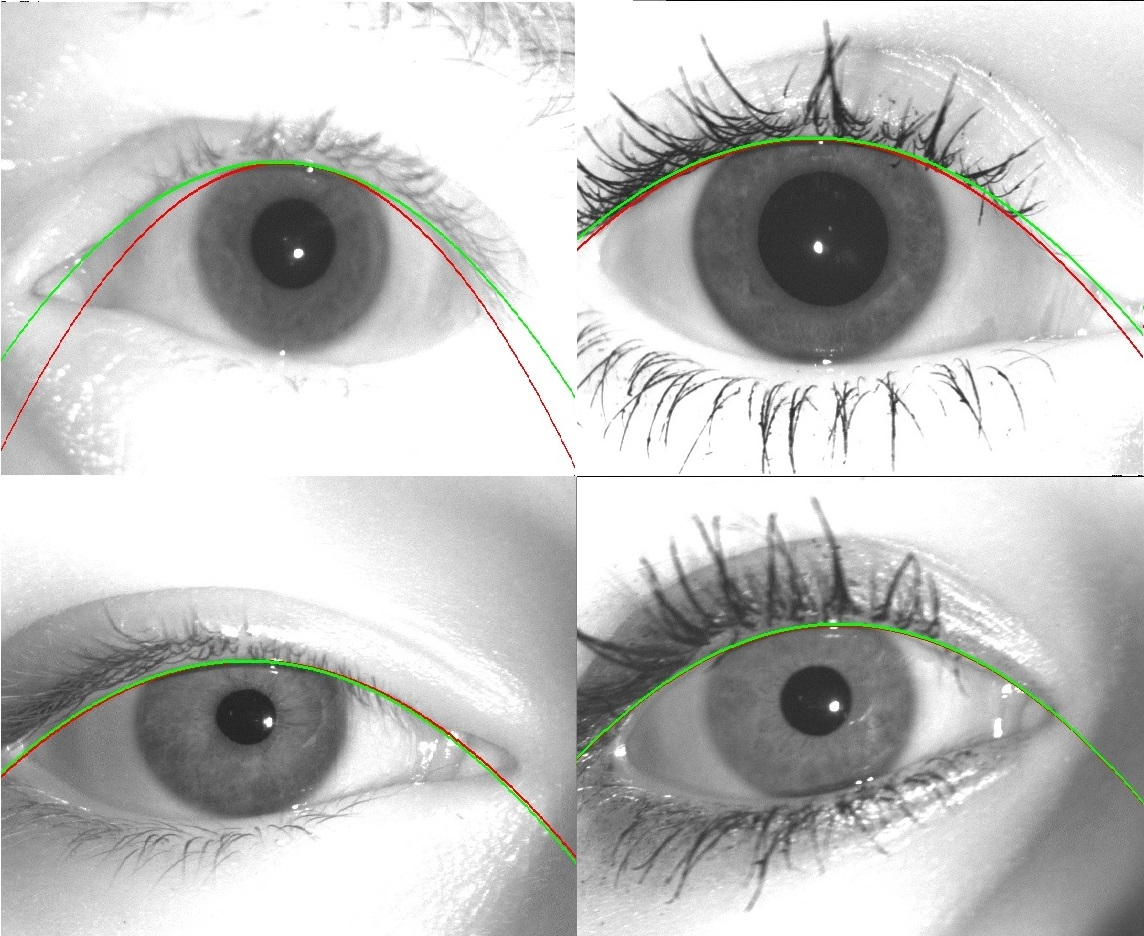
\includegraphics[width=0.6\linewidth]{compare.jpg}
	
	\caption{Сравнение результата с эталоном. Красная линия~--- эталон, зеленая~--- результат алгоритма.}
	
	\label{fig:compare}
	
\end{figure}

\subsection{Распределение ошибки}
Распределение величины ошибки на всей базе изображений $LG4000$ (2864 изображения) на рис.~\ref{fig:gist}. 

\begin{figure}[h]
	\centering
	
	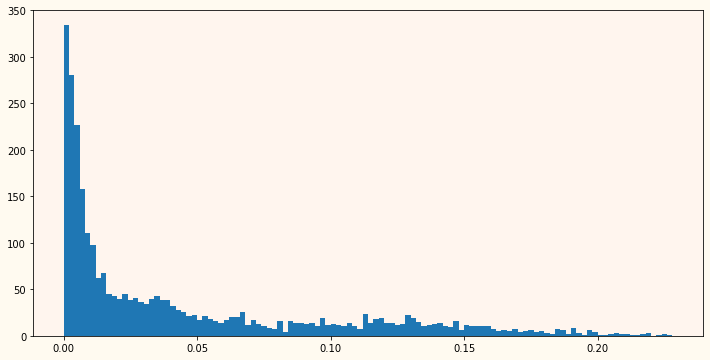
\includegraphics[width=0.67\linewidth]{gist.jpg}
	\caption{Распределение величины ошибки на базе $LG4000$.}
	
	\label{fig:gist}
\end{figure}

Средняя величина ошибки на всей выборке~---~$4,8\%$, медианная ошибка~---~$2,1\%$.


\subsection{Сравнение результатов с другими методами}
Также рассчитаем величину ошибки $dist$~\eqref{dist} и ее распределение (рис.~\ref{fig:gist2}).

\begin{figure}[h]
	\centering
	
	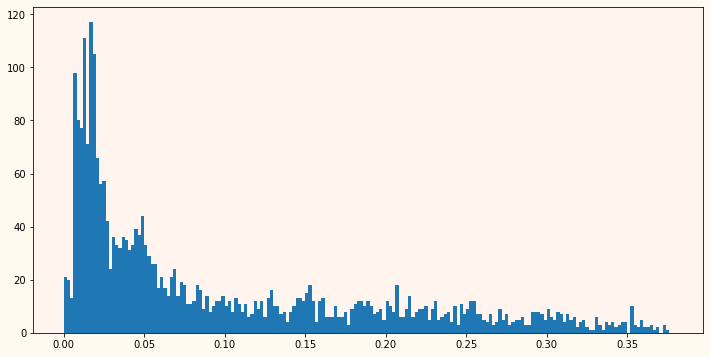
\includegraphics[width=0.67\linewidth]{gist2.jpg}
	\caption{Распределение величины ошибки $dist$ на базе $LG4000$.}
	
	\label{fig:gist2}
\end{figure}

Средняя величина ошибки $dist$ на всей базе изображений~---~$12,2\%$, медианная ошибка~---~$5,8\%$.

В~Таблице~\ref{Tab:1} дано сравнение результатов работы алгоритма с другими методами, упомянутыми в разделе~\ref{task}.

\begin{table}[h]
	\centering
	%\begin{tabular}{l|l|l|l}
	\begin{tabular}{ccc}
		\hline Модель & Ошибка,~\%  &   \\
		\hline Пр. Хафа \cite{Wildes} & 19,4 &  \\
		Ф. Собела + IDO \cite{KP} & 7,7 &   \\
		Ф. Собела + пр. Хафа \cite{Adam_1} & 11,5 &  \\
		Ф. Габора + IDO \cite{KKX} & 14,2 &   \\
		\hline
		\textbf{Исследуемая модель}&   \textbf{12,2}&     \\
		\hline 
	\end{tabular}

	\caption{Сравнение точности определения крайней верхней точки верхнего века существующими современными алгоритмами с исследуемой моделью}
	\label{Tab:1}
\end{table}

Нетрудно заметить, что даже эта оценка качества даёт сопоставимый результат.
%%%%%%%%%%%%%%%%%%%%%%%%%%%%%%%%%%%%%%%%%%%%%%%%%%%%%


\newpage
\section{Заключение}

Предложен метод, разработан и протестирован алгоритм выделения века как параболической кривой. Сравнение с разметкой эксперта показывает состоятельность подхода и хорошее качество результата. Аналогичные выводы можно сделать из сравнения результатов работы предложенного метода с существующими алгоритмами. Возможными направлениями развития могут быть: сужение потенциальной области поиска искомых параметров, уменьшение шума ресниц и оптимизация работы алгоритма для неожидаемых углов наклона изображения.

%%%%%%%%%%%%%%%%%%%%%%%%%%%%%%%%%%%%%%%%%%%%%%%%%%%%%


\newpage

\bibliographystyle{gost71s}
\bibliography{mylib}
\nocite{GV}

\end{document}